% !TeX encoding = UTF-8
% !TeX spellcheck = de_DE

%% Dies gibt Warnungen aus, sollten veraltete LaTeX-Befehle verwendet werden
\RequirePackage[l2tabu, orthodox]{nag}
\documentclass[utf8,biblatex]{lni}
\usepackage[utf8]{inputenc}
\usepackage[T1]{fontenc} % T2A for cyrillics
\bibliography{../Dokumentation/Bibliography, ../Dokumentation/snik}
\usepackage{todonotes}

%% Schöne Tabellen mittels \toprule, \midrule, \bottomrule
\usepackage{booktabs}

%% Akronyme
\usepackage{acronym}

% AURL
\PassOptionsToPackage{bookmarks=false}{hyperref} % prevent option clash for hyperref with lni
\usepackage{aurl}
\daurl{bb}{http://www.snik.eu/ontology/bb/}
\daurl{meta}{http://www.snik.eu/ontology/meta/}

%% Plots
\usepackage{tikz}
\usepackage{pgfplots}
\pgfplotsset{compat=1.18}
\usepgfplotslibrary{groupplots}

\begin{document}
%%% Mehrere Autoren werden durch \and voneinander getrennt.
%%% Die Fußnote enthält die Adresse sowie eine E-Mail-Adresse.
%%% Das optionale Argument (sofern angegeben) wird für die Kopfzeile verwendet.
\title[Question Answering auf SNIK]{Question Answering auf einer Ontologie des Informationsmanagements im Krankenhaus}
%%%\subtitle{Untertitel / Subtitle} % falls benötigt
\author[Hannes R. Brunsch]% \and Konrad Höffner]
{Hannes R. Brunsch\footnote{Wilhelm-Ostwald-Schule, Gymnasium der Stadt Leipzig, Willi-Bredel-Straße 15, 04279 Leipzig, Deutschland \email{hrbrunsch@gmail.com}}}
%\and  Konrad Höffner\footnote{Universität Leipzig, Institut für Medizinische Informatik, Statistik und Epidemiologie, Härtelstraße 16--18, 04107 Leipzig, Deutsche \email{konrad.hoeffner@uni-leipzig.de}}}
\startpage{1} % Beginn der Seitenzählung für diesen Beitrag
\editor{Gesellschaft für Informatik}    % Namen der Herausgeber
\booktitle{Studierendenkonferenz Informatik} % Name des Tagungsband; optional Kurztitel
\yearofpublication{2023}
%%%\lnidoi{18.18420/provided-by-editor-02} % Falls bekannt
\maketitle

\begin{abstract}
Mit der beständig fortschreitenden Digitalisierung wird es immer wichtiger, auch das Wissen über das Informationsmanagement,
also die Verarbeitung von Informationen und die dazu nötigen Schritte digital und strukturiert erreichbar zu machen.
Die Ontologie SNIK enthält Wissen aus dem Bereich des Informationsmanagements im Krankenhaus und soll künftig auch bei dem Studium der Medizininformatik helfen.
Um das Wissen mittels geschriebener natürlicher Sprache verwendbar zu machen, wird Question Answering vorgeschlagen.
Hierfür gibt es verschiedene Systeme, viele sind allerdings auf bestimmte Wissensbasen spezialisiert.
Mittels dem hier ausgewählten System QAnswer ist es möglich, die Ontologie mit ausreichender Genauigkeit zu durchsuchen.
Die Antworten werden anhand eines vorher definierten Fragenkataloges auf ihre Genauigkeit hin überprüft und bewertet.
Das System ist über die SNIK-Website frei erreichbar.
\end{abstract}

\begin{keywords}
Semantic Web \and Question Answering \and Knowledge Graph Question Answering \and Closed Domain Question Answering
\end{keywords}

\section{Einleitung}
Das semantische Netz des Informationsmanagements im Krankenhaus (SNIK) ist eine
die Domäne des Informationsmanagements im Krankenhaus betreffende Ontologie \cite{domaene}.
Sie behandelt Wissen über Krankenhausinformationssysteme und deren Management.
Dieses wurde aus drei Lehrbüchern \cite{bb,ob,he} und einem Interview \cite{ciosurvey} manuell extrahiert und im Resource Description Format (RDF) modelliert.

Momentan müssen Studierende der Medizininformatik, die nach Wissen suchen, auf eine der drei folgenden Optionen zurückgreifen.
Jede dieser Möglichkeiten hat jedoch große Nachteile.
Der RDF-Browser gibt nur ein sehr beschränktes Ergebnis aus, serialisiertes RDF selbst zu lesen ist für Laien schwer.
Eine existierende Visualisierung als Graph ist zu unübersichtlich, um eine spezifische Frage schnell zu beantworten.
Zuletzt gibt es noch die Möglichkeit, die Ontologie mithilfe der Abfragesprache SPARQL Protocol and RDF Query Language (SPARQL) zu durchsuchen.
Hier gibt es jedoch einen erheblichen Zeitaufwand für die Studierenden, da sie sich erst in die Syntax SPARQLs und das Vokabular SNIKs einarbeiten müssen.

Daraus ergibt sich das Problem, dass keine der momentan existierenden Lösungen intuitiv genug funktioniert.
Alle benötigen beim Nutzer eine gewisse Einarbeitungszeit.
Die existierenden Lösungen liefern zudem nicht übersichtlich ausreichend Informationen.
Ein Ansatz für eine mögliche neue Lösung ist Question Answering (QA), die Beantwortung von in natürlicher Sprache gestellten Fragen.

Das Wissen zum Informationsmanagement im Krankenhaus ist komplex und oft nur schwer greifbar.
Es liegt in Form von Lehrbüchern, aber auch in SNIK vor.

Es ist ein großer Mehraufwand für Studierende, sich ganze Kapitel oder gar Bücher durchzulesen, um einzelne Fragen zu beantworten.
Viele verfügen nicht über die Kenntnisse, SNIK effektiv zu verwenden.
Als Folge müssen sie bei Fragen oft ihren Professor oder andere Studierende hinzuziehen.
QA-Systeme sind immer leicht erreichbar und können sofort antworten.

\section{Grundlagen}

\subsection{SNIK}

Die in RDF modellierten Quellen SNIKs werden alle in je einer Ontologie abgebildet.
Teilontologien werden mittels der Metaontologie modelliert und miteinander verbunden.
Deshalb ist SNIK sowohl eine Wissensbasis als auch Ontologie:
Es werden zwar keine einzelnen Krankenhäuser abgebildet, aber das Wissen aus verschiedenen Lehrbüchern, die im allgemeinen davon handeln.
Die Metaontologie gibt allem eine einer Wissensbasis ähnliche Struktur.

\begin{figure}[h]
  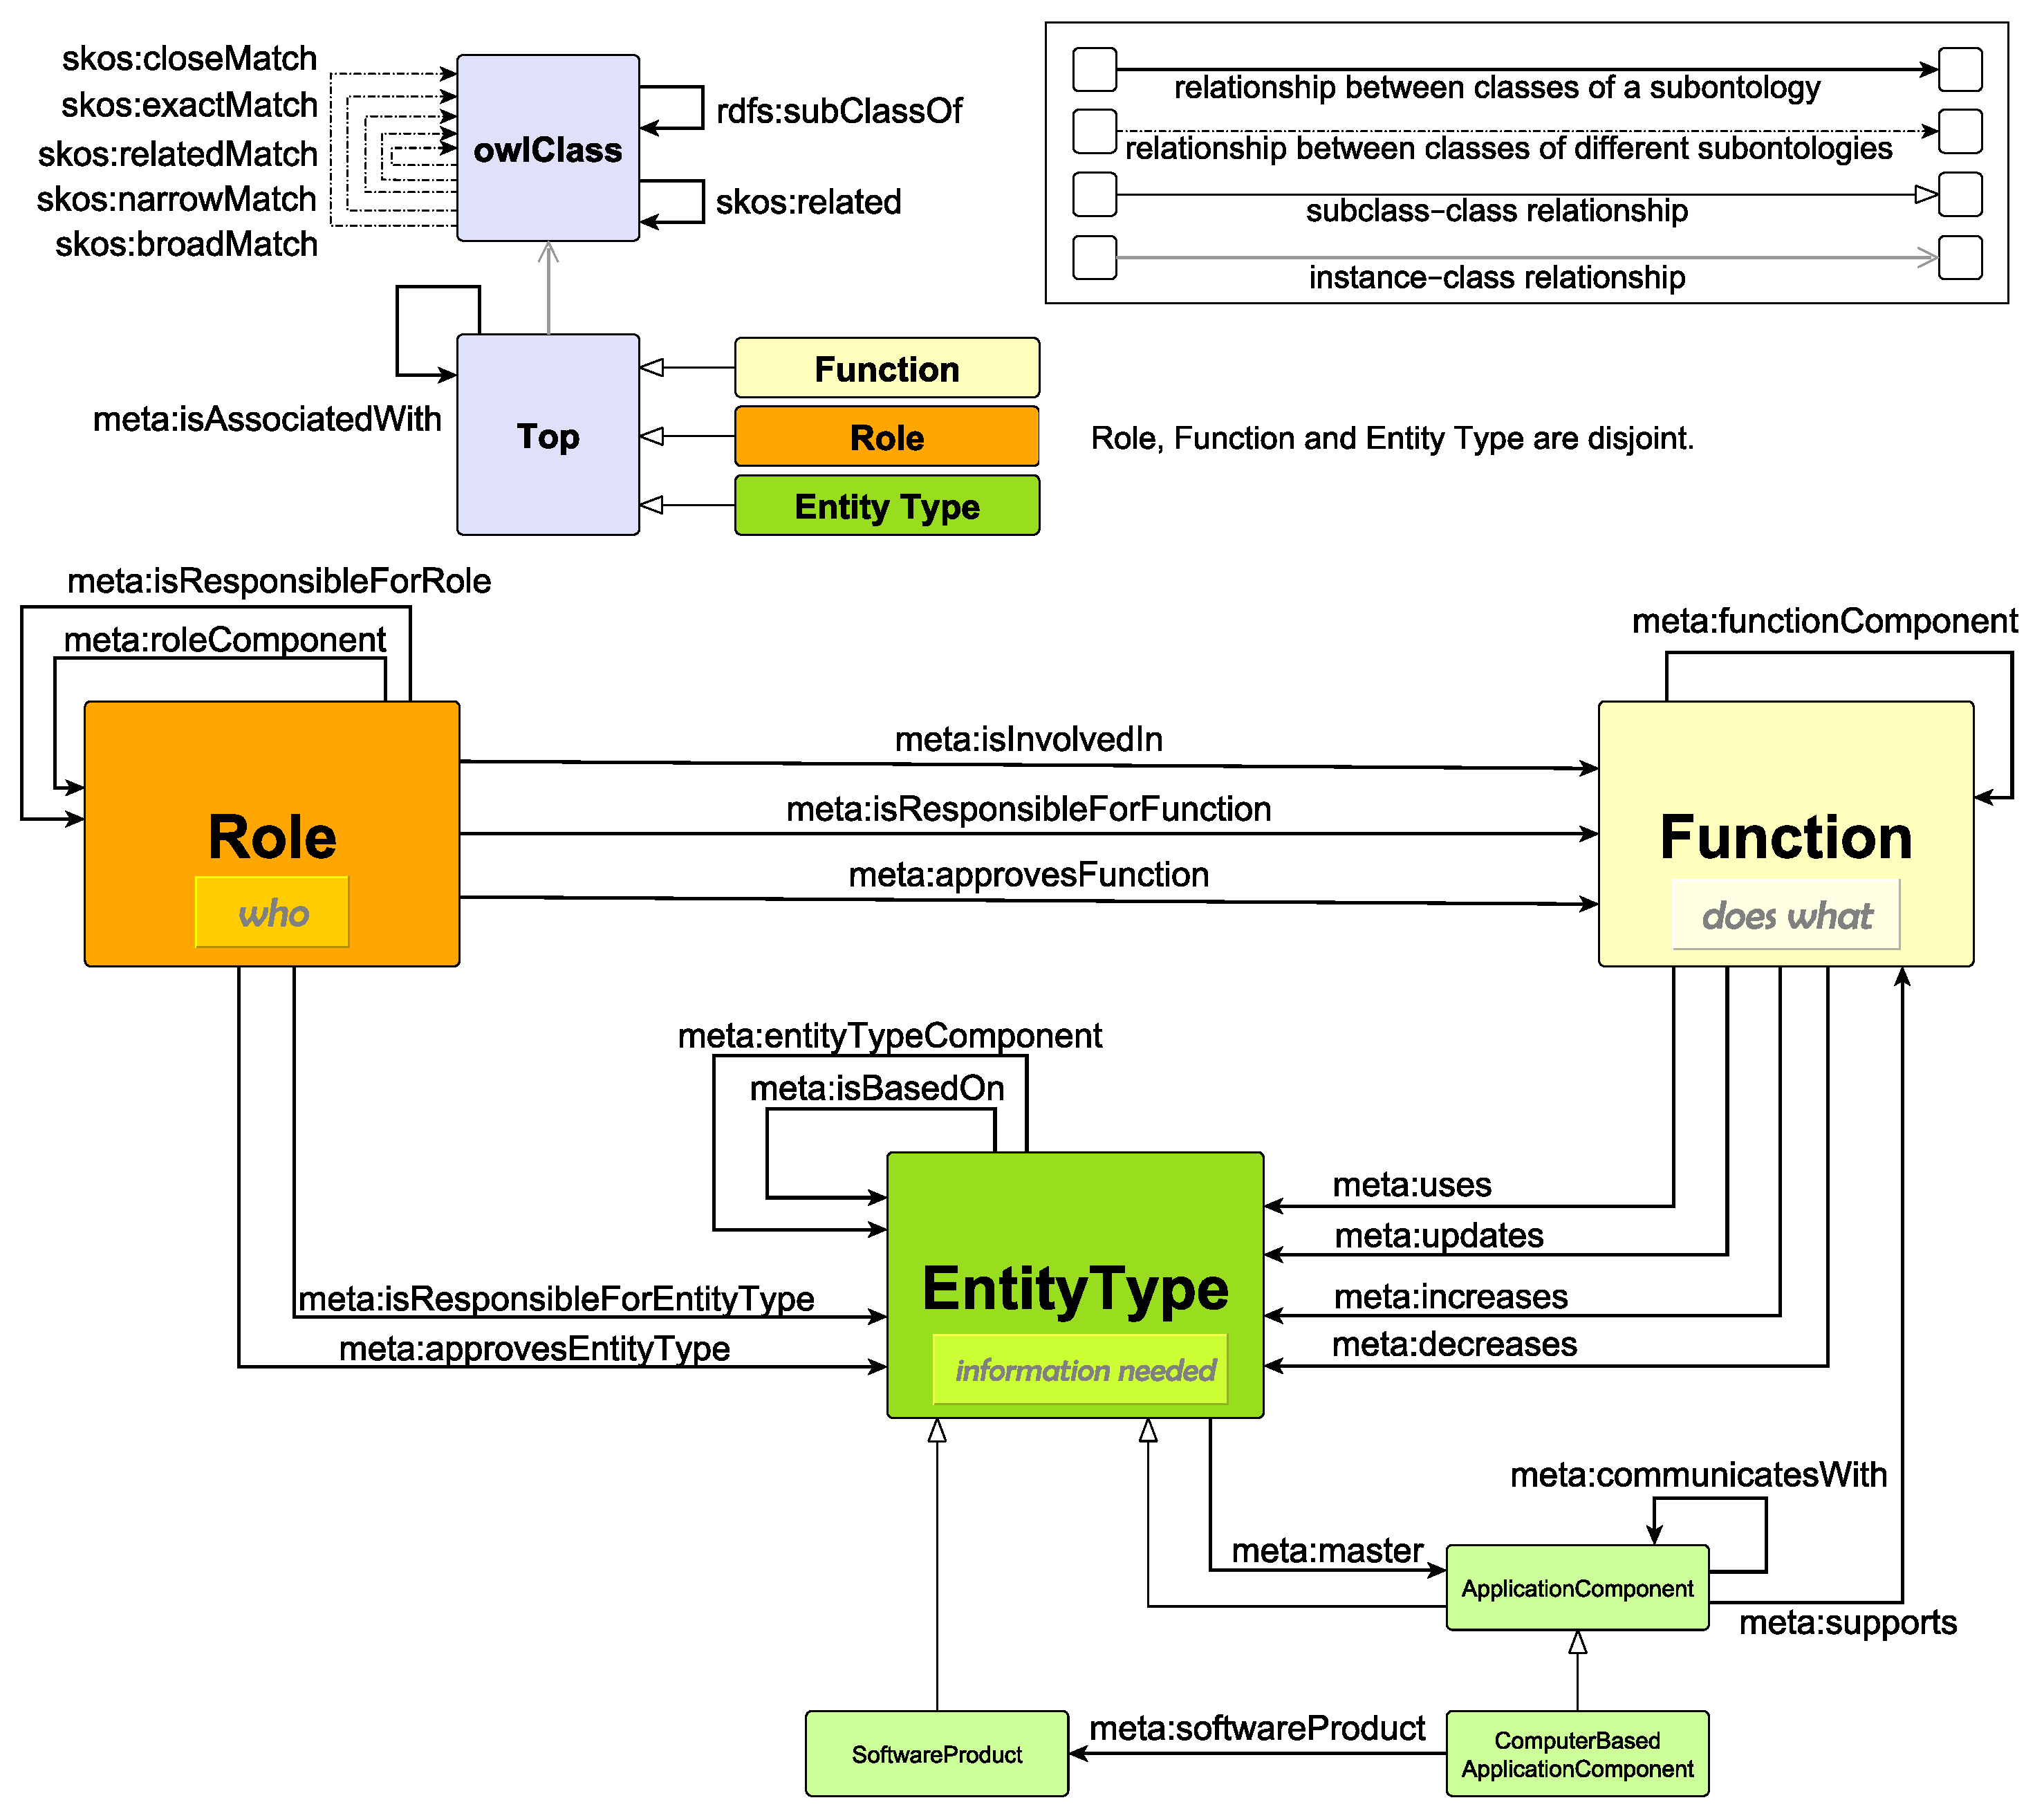
\includegraphics[width=\linewidth]{../Dokumentation/Images/snik-metamodel-V10.pdf}\label{fig:snik-metamodel}
  \caption[SNIK Metamodell Version 10]{Das SNIK Metamodell Version 10. Quelle: \url{https://www.snik.eu/public/SNIK_Metamodell_V10.svg}}
\end{figure}
In \cref{fig:snik-metamodel} ist die Metaontologie dargestellt.
Von den drei Klassen \emph{Role}, \emph{EntityType} und \emph{Function} stammen alle anderen Klassen der Teilontologien ab.
Sie beschreiben respektive Personen, Informationen im Krankenhaus und Funktionen.
Alle in der Ontologie vorhandenen Prädikate sind in der Metaontologie definiert.
So sind zwischen den in verschiedenen Teilontologien ähnliche Ressourcen in Relation gesetzt und die Beziehungen zwischen Ressourcen in den einzelnen Teilontologien dargestellt.

\subsection{QA-Systeme}

Question Answering (Fragebeantwortung) behandelt die Beantwortung von Benutzerfragen \citep{qadefinition}.
Ein QA-System muss eine Frage analysieren, eine oder mehrere Antworten bereitstellen und dem Nutzer diese präsentieren.
Die Fragen sind in natürlicher Sprache gestellt.

Das QA-Leaderboard \citep{leaderboardinproceedings} hat es sich zur Aufgabe gemacht,
dem häufig als sehr uneinheitlich und unübersichtlich \citep{diefenbachkbqa} beschriebenen Feld des QA auf Wissensbasen und Ontologien (KGQA) eine vereinheitliche Liste mit verfügbaren QA-Systemen zu geben.
Hier werden Fragenkataloge wie QALD-9 \cite{qald9} als Benchmarks auf die verschiedenen KGQA-Systeme angewendet und die Ergebnisse aufgezeichnet.
Mithilfe dieses Projektes konnten mehrere Kandidaten für das Question Answering auf SNIK ausgewählt werden.

Das System gAnswer \cite{ganswerapproach} spaltet Fragen in Syntaxbäume auf und vergleicht später Subgraphen der möglichen Antworten, jedoch kommt es bei der komplexen Vorbereitung und Umwandlung der Daten der Ontologie immer wieder zu Fehlern.
DeepPavlov \cite{deeppavlov} ist ein hochmodulares, hochflexibles System mit der Oberfläche eines Chatbots, leider aber nicht mit eigenen Daten nutzbar.
TeBaQA \cite{tebaqa} analysiert die Struktur einer Frage und versucht, sie einer Vorlage zuzuordnen, wodurch dann die SPARQL-Abfrage erstellt wird.
Auch hier gibt es nicht behebbare Probleme bei der Einrichtung des Systems für SNIK.
Betrachtet wird außerdem AskNow QA \cite{asknow}, welches mittels PoS-Tagging versucht, eine \emph{normalisierte Fragenstruktur} herzustellen und darüber eine SPARQL-Abfrage zu generieren.
Aufgrund des Entity Linkings kann allerdings momentan nur DBpedia verwendet werden.

Hier wird QAnswer KG \cite{qanswer} verwendet.
Dieses fokussiert sich auf die Verfügbarkeit von Question Answering für individuelle Datensätze,
also auf das Problem der fehlenden Portabilität.
Viele andere QA-Systeme fokussieren sich auf große Wissensbasen wie DBpedia und WikiData \cite{qald9plus},
welche große Mengen an Daten zur Verfügung stellen.
Bei kleineren Datenmengen gibt es aber das Problem, das häufig zu wenige Trainingsdaten für das Abstimmen der Algorithmen auf die Wissensbasen zur Verfügung stehen, als dass man ein Sprachmodell zum Verstehen natürlichsprachiger Fragen von Grund auf trainieren kann.
Deshalb verwendet QAnswer Sprachmodelle, welche schon vorher viel auf normale Texte trainiert wurden und nun mittels Nutzerfragen präzisiert werden.

QAnswer erstellt alle für die gegebene Frage möglichen Kombinationen von Wörtern der Frage (N-Gramme), nachdem die sogenannten \emph{Stoppwörter}, eine vorgefertigte Liste an z.B. Artikeln, entfernt wurden.
Diese N-Gramme versucht es dann auf mögliche Repräsentationen im Datensatz mittels Labels zu matchen.
Daraus werden viele mögliche SPARQL-Abfragen kreiert, welche anhand bestimmter Kriterien einen \emph{Confidence}-Wert zwischen $0\%$ und $100\%$ erhalten.
Die SPARQL-Abfrage mit dem höchsten Wert wird ausgewählt, ist er größer als $50\%$ gilt die Antwort als richtig, sonst wird keine ausgegeben.
SPARQL ist ein World Wide Web Consortium (W3C)-Standard als Abfragesprache für RDF.

Bei der Frage \enquote{How can quality of HIS be evaluated?} werden beispielsweise die Wörter \enquote{How}, \enquote{can}, \enquote{of} und \enquote{be} nicht betrachtet, sie bieten bei der Suche nach passenden Kombinationen kaum einen Mehrwert.
Die Wörter \enquote{quality}, \enquote{HIS} und \enquote{evaluated} werden nun auf alle mögliche Arten kombiniert, hier sollten die Kombinationen \enquote{quality HIS} und \enquote{evaluated} herauskommen, welche die Ressource \aurl{bb}{EvaluationMethod} finden und das Prädikat \aurl{rdfs}{subClassOf} implizieren muss.
Diese Frage wurde nie richtig beantwortet, da die Lösung anhand der Daten der Ontologie wenig plausibel erscheint.

\section{Anpassung von QAnswer KG an SNIK}

QAnswer KG versucht, sich auf eine Antwort zu konzentrieren und stellt nur die als am besten bewertete SPARQL-Abfrage dar.
Hier wird das Problem der Ambiguität deutlich, da bei der Frage \enquote{What is the chief information officer responsible for?} sowohl
\aurl{meta}{isResponsibleForEntityType}, \aurl{meta}{isResponsibleForFunction} und \aurl{meta}{isResponsibleForRole} gemeint sein können.
Der Ansatz für die Lösung dieses Problems ist es, das System alle drei ausführen zu lassen, oder ihm das zumindest zu ermöglichen.

Dies kann zum Beispiel über SPARQL 1.1 Property Paths realisiert werden.
In diesem Fall erlauben Property Paths dem Prädikat, in der Abfrage verschiedene Ressourcen darstellen zu können.
Es werden letztendlich drei Abfragen ausgeführt, eine für jede mögliche Kombination der Attribute, also hier einmal pro Prädikat.
Statt allein \aurl{meta}{isResponsibleForEntityType} steht durch die Nutzung von Property Paths nun \aurl{meta}{isResponsibleForRole} | \aurl{meta}{isResponsibleForFunction} | \aurl{meta}{isResponsibleForEntityType} dort.
Jedoch kann QAnswer keine Property Paths aufstellen, weshalb diese Option zur Lösung des Ambiguitätsproblems wegfällt.

Eine andere Möglichkeit, die obige Frage mittels einer SPARQL-Abfrage zu beantworten, ist mittels der \aurl{rdfs}{subPropertyOf}-Beziehung.
Diese regelt die Hierarchie von Properties.
So sind die drei, welche hier alle in einer Abfrage zusammengefasst werden sollen, alle ein Subproperty von \aurl{meta}{subPropertyOf}.

Deshalb müssen vor dem Training die \aurl{rdfs}{subPropertyOf}+-Beziehung materialisiert werden.
Das heißt es werden alle transitiven Subpropertybeziehungen zu Trainingszwecken mittels dem SPARQL-Befehl \texttt{CONSTRUCT} zu direkten Subklassenbeziehungen umgeformt.\footnote{Verwendete n-Tripel-Datei verfügbar unter:\\\url{https://github.com/Yagnap/BeLL-Question-Answering-auf-Linked-Data-SNIK/blob/main/Data/qanswerset.nt}}

Zusätzlich werden auch die \aurl{rdfs}{subClassOf}+-Beziehungen materialisiert.
Dies muss geschehen, da die Antworten für manche Textbuchfragen alle transitiven Subklassen sind.

Durch die Materialisierung kann beispielsweise für die Frage \enquote{How can quality of HIS be evaluated?}
die Klasse \aurl{bb}{CaseStudy} gefunden werden, obwohl diese eine direkte Subklasse von \aurl{bb}{QualitativeEvaluationMethod} ist,
welche wiederum eine direkte Subklasse von \aurl{bb}{EvaluationMethod} ist, welche in der Abfrage gesucht wird.
Die Abfrage, welche die \aurl{rdfs}{subClassOf+}-Beziehung kann nicht durch QAnswer generiert werden, die materialisierte \aurl{rdfs}{subClassOf} jedoch schon.

Wenn keine Lösung für die Frage gefunden wird, gibt es als Ausgabe meist die Ressource selbst, also zum Beispiel \aurl{bb}{ChiefInformationOfficer}.
Dies kann zwar nützlich, aber auch verwirrend sein und soll mithilfe von Training verhindert werden.
Praktisch für die Lokalisierung der Fehler ist die Funktion, sich alle generierten Anfragen anzeigen zu lassen.
Somit kann erahnt werden, warum es das macht, was es macht.

Mit der Konfiguration an sich können bereits viele Fehler behoben werden.
Unter den Stoppwörtern sind häufig verwendete Präpositionen, Konjunktionen, Verben oder Füllwörter wie \enquote{and} oder \enquote{many}.
Hier muss diese Liste allerdings so modifiziert werden, dass das Wort \texttt{for} nicht mehr darin vorkommt, denn ohne es können Prädikate wie \enquote{responsible for} schwer erkannt werden,
besonders, da die beiden Wörter oft getrennt im Satz vorkommen.
Entfernt wurden auch \texttt{define} und \texttt{describe}, da auch diese in Labels vorkommen.
Zu den \emph{Hidden Properties} wurde \aurl{rdfs}{subClassOf} hinzugefügt.
Hidden Properties sind solche, die nicht explizit in der Frage benutzt werden, aber trotzdem impliziert werden können.
Es wurde \aurl{skos}{altLabel} als weiteres Label für Ressourcen hinzugefügt, sodass QAnswer auch diese beachtet.
Die Mappings müssen auch dahingehend verändert werden, als dass \aurl{skos}{definition}
und \aurl{rdfs}{comment} als Beschreibung hinzugefügt werden.
Die Definition wird auch bei den Ergebnissen angezeigt, sodass es bei Ergebnissen von Fragen nach der Definition als richtig erachtet wird, wenn die zu definierende Ressource richtig erkannt wurde.

Es gibt auch die Möglichkeit, direkt Wörter als Aliase für URIs zu nutzen.
Bei den \emph{Property Mappings} können URIs und dafür stehende Lexikalisierungen in Abhängigkeit gebracht werden, wie bei einem Wörterbuch.
Dies wird hier für \enquote{phases} und \enquote{methods} bei \aurl{meta}{updates} sowie \enquote{tasks} und \aurl{meta}{functionComponent} gemacht.
Für \aurl{meta}{entityTypeComponent} wird \enquote{facets} hinzugefügt.
Lexikalisierungen funktionieren ähnlich wie alternative Labels.
Notwendig ist es aufgrund der Funktionsweise QAnswers; ohne Lexikalisierungen weiß das Programm nicht, wofür die Ressourcen stehen.
Da die Properties in SNIK sehr allgemein gehalten sind, fehlen oft Labels mit ausreichend präziser Formulierung, mithilfe derer QAnswer auf die Ressource als Teil der Antwort schließen kann.
Für diese stehen die Lexikalisierungen zur Verfügung.

\section{Benchmark}

Die Performance des Systems soll anhand eines Benchmarks aus Frage-Antwort-Paaren untersucht werden.
Die Frage liegt hierbei in natürlicher Sprache, die Antwort als SPARQL-Abfrage vor.
100 Fragen sollen als Testdatensatz, der immer wieder abgefragt wird, dienen,
alle anderen Fragen sollen in Schritten von 10 Fragen QAnswer trainieren und somit die Abhängigkeit von den Indikatoren \emph{Genauigkeit} (\emph{precision}), \emph{Trefferquote} (\emph{recall}) und \emph{F-Maß} (\emph{F-score}) zur Anzahl der Fragen geben.

QAnswer kann mittels Nutzerfragen trainiert werden.
Herausgefunden werden soll der Einfluss der Anzahl der Nutzerfragen auf die Qualität der Antworten und somit das mögliche Finden eines Optimums.
Weiterhin wird dies einmal mit und einmal ohne Lehrbuchfragen geschehen, da auch der Einfluss von deren erhöhter Schwierigkeit auf die Ergebnisse bestimmt wird.

Das Lehrbuch selbst \cite{bb} enthält am Ende von Kapiteln bereits Fragen, welche das Gelernte zusammenfassen sollen.
Ausgehend von \cite{arneba} wurden die Fragen anhand ihrer Eignung für das Training klassifiziert.
Es wurden nur Fragen in Betracht gezogen, die Anforderungsbereich 1 entsprechen, also Fakten wiedergeben sollen und nicht z.B. zusammenfassen.
Nicht alle Fragen haben Antworten in der Ontologie, diese wurden auch herausgefiltert.
Der Rest wurde in SPARQL-Abfragen umgewandelt.
Insgesamt gibt es 36 Lehrbuchfragen und zugehörige Antworten.

Da diese Fragen sowohl sehr kompliziert gestellt als auch viel zu wenige sind, werden aus dem Datenbestand der Teilontologie auch Fragen nach dem Schema \emph{Subjekt bzw. Objekt - Prädikat - Objekt bzw. Subjekt} gestellt.
Diese und die zugehörigen Antworten lassen sich mittels SPARQL-Abfragen automatisch erstellen.
Daraus entstehen 621 Fragen nach dem Subjekt und 374 Fragen nach dem Objekt, also insgesamt 995 weitere Frage-Antwort-Paare, mit denen das Training beginnen kann.

\section{Ergebnisse}

Das Frage-Antwort-Set aus dem Lehrbuch wurde in zwei Hälften geteilt, eine zum Training und eine zum Testen.
Die Fragen wurden randomisiert in die Gruppen eingeteilt, sodass 18 im Trainingsdatensatz und 18 im Testdatensatz sind.
Die Frage \enquote{How can quality of HIS be evaluated?} ist beispielsweise im Testsatz, wurde nie richtig beantwortet und hat deshalb immer eine Genauigkeit und Trefferquote von $0\%$ und zu Evaluationszwecken hier auch ein F-Maß von $0\%$.

Von den automatisch generierten Paaren wurden 100 für das Testen und 895 für das Training genutzt.
Das Training verläuft so ab, dass dem System automatisiert pro Schritt zehn weitere automatisch generierte Paare aus dem Trainingsdatensatz gegeben werden,
wodurch jede Runde mit zehn zusätzlichen Fragen trainiert wird.
Der Trainingssatz der Lehrbuchfragen wird in der ersten Runde nicht mit verwendet,
in der zweiten Runde werden von Anfang an alle Textbuchfragen verwendet.

Dann wird QAnswer mithilfe der API-Methode trainiert.
Auf das trainierte System wird der Testdatensatz zur Evaluierung angewandt.
Über eine API-Abfrage wird die Antwort mit dem höchsten Confidence-Wert, eine SPARQL-Abfrage, geholt und auf dem SPARQL-Endpunkt von SNIK ausgeführt.
Die Antworten der richtigen Lösung wurden schon vorher gespeichert und werden nun mit denen der Abfrage von QAnswer verglichen.
Dann wird das trainierte Modell zurückgesetzt, die gegebenen Frage-Antwort-Paare bleiben jedoch erhalten.

% PLOTS
\begin{figure}%[h!]
  \centering
  \begin{tikzpicture}
    \begin{groupplot}[
        group style = {
          xlabels at = edge bottom,
          ylabels at = edge left,
          horizontal sep = 2cm,
          vertical sep = 2cm,
          group size = 2 by 3,
        },
        width = 0.5\linewidth
        ]

        % F-Score
        \nextgroupplot[
          title=F-Maß autogenerierte Fragen,
          grid=major, % Display a grid
          grid style={dashed,gray!30}, % Set the style
          xlabel=Anzahl der generierten Trainingsfragen, % Set the labels
          ylabel=F-Maß,
          label style={font=\scriptsize},
					xtick distance=200,
					mark size=0.6,
          title style={
            at={(0.5,0.95)}, above, yshift=0,
          },
          xmin=0,xmax=895,
          ymin=0,ymax=1,
        ]
        \addplot table[x=Anzahl Trainingsfragen,y=F-Score,col sep=comma] {../../Data/Tabellen/Training-Auswertung/generated.csv};
        \addplot table[x=Anzahl Trainingsfragen,y=F-Score,col sep=comma] {../../Data/Tabellen/Training-Auswertung/generated-withtb.csv}; 

        % F-Score TB
        \nextgroupplot[
          title=F-Maß Lehrbuchfragen,
          grid=major, % Display a grid
          grid style={dashed,gray!30}, % Set the style
          xlabel=Anzahl der generierten Trainingsfragen, % Set the labels
          ylabel=F-Maß,
          label style={font=\scriptsize},
					xtick distance=200,
					mark size=0.6,
          title style={
            at={(0.5,0.95)}, above, yshift=0,
          },
          xmin=0,xmax=895,
          ymin=0,
        ]
        \addplot table[x=Anzahl Trainingsfragen,y=F-Score,col sep=comma] {../../Data/Tabellen/Training-Auswertung/textbook-av.csv};
        \addplot table[x=Anzahl Trainingsfragen,y=F-Score,col sep=comma] {../../Data/Tabellen/Training-Auswertung/textbook-av-withtb.csv}; 
        
        % Precision
        \nextgroupplot[
          title=Genauigkeit autogenerierte Fragen,
          grid=major, % Display a grid
          grid style={dashed,gray!30}, % Set the style
          xlabel=Anzahl der generierten Trainingsfragen, % Set the labels
          ylabel=Genauigkeit,
					label style={font=\scriptsize},
					xtick distance=200,
					mark size=0.6,
          title style={
            at={(0.5,0.95)}, above, yshift=0,
          },
          xmin=0,xmax=895,
          ymin=0,ymax=1,
        ]
        \addplot table[x=Anzahl Trainingsfragen,y=Precision,col sep=comma] {../../Data/Tabellen/Training-Auswertung/generated.csv};
        \addplot table[x=Anzahl Trainingsfragen,y=Precision,col sep=comma] {../../Data/Tabellen/Training-Auswertung/generated-withtb.csv}; 

        % Precision TB
        \nextgroupplot[
          title = Genauigkeit Lehrbuchfragen,
          grid=major, % Display a grid
          grid style={dashed,gray!30}, % Set the style
          xlabel=Anzahl der generierten Trainingsfragen, % Set the labels
          ylabel=Genauigkeit,
          label style={font=\scriptsize},
					xtick distance=200,
					mark size=0.6,
          title style={
            at={(0.5,0.95)}, above, yshift=0,
          },
          xmin=0,xmax=895,
          ymin=0,
        ]
        \addplot table[x=Anzahl Trainingsfragen,y=Precision,col sep=comma] {../../Data/Tabellen/Training-Auswertung/textbook-av.csv};
        \addplot table[x=Anzahl Trainingsfragen,y=Precision,col sep=comma] {../../Data/Tabellen/Training-Auswertung/textbook-av-withtb.csv}; 
        
        % Recall
        \nextgroupplot[
          title=Trefferquote autogenerierte Fragen,
          grid=major, % Display a grid
          grid style={dashed,gray!30}, % Set the style
          xlabel=Anzahl der generierten Trainingsfragen, % Set the labels
          ylabel=Trefferquote,
          label style={font=\scriptsize},
					xtick distance=200,
					mark size=0.6,
          title style={
            at={(0.5,0.95)}, above, yshift=0,
          },
          xmin=0,xmax=895,
          ymin=0,ymax=1,
        ]
        \addplot table[x=Anzahl Trainingsfragen,y=Recall,col sep=comma] {../../Data/Tabellen/Training-Auswertung/generated.csv};
        \addplot table[x=Anzahl Trainingsfragen,y=Recall,col sep=comma] {../../Data/Tabellen/Training-Auswertung/generated-withtb.csv}; 

        % Recall TB
        \nextgroupplot[
          title=Trefferquote Textbuchfragen,
          grid=major, % Display a grid
          grid style={dashed,gray!30}, % Set the style
          xlabel=Anzahl der generierten Trainingsfragen, % Set the labels
          ylabel=Trefferquote,
          label style={font=\scriptsize},
					xtick distance=200,
					mark size=0.6,
          title style={
            at={(0.5,0.95)}, above, yshift=0,
          },
          xmin=0,xmax=895,
          ymin=0,
          legend style={at={(-0.2,-0.3)},anchor=north}, % Put the legend below the plot
        ]
        \addplot table[x=Anzahl Trainingsfragen,y=Recall,col sep=comma] {../../Data/Tabellen/Training-Auswertung/textbook-av.csv};
        \addlegendentry{Training ohne Lehrbuchfragen}
        \addplot table[x=Anzahl Trainingsfragen,y=Recall,col sep=comma] {../../Data/Tabellen/Training-Auswertung/textbook-av-withtb.csv}; 
        \addlegendentry{Training mit Lehrbuchfragen}

        \legend{Training ohne Lehrbuchfragen,Training mit Lehrbuchfragen}
    \end{groupplot}
  \end{tikzpicture}
  \caption{F-Maß, Genauigkeit, und Trefferquote von Lehrbuchtestfragen und automatisch generierten Testfragen in Abhängigkeit zur Anzahl und Zusammensetzung der Trainingsfragen.}
\end{figure}

\begin{figure}
  \begin{tikzpicture}
    \begin{groupplot}[
      group style = {
        xlabels at = edge bottom,
        ylabels at = edge left,
        horizontal sep = 2cm,
        vertical sep = 2cm,
        group size = 2 by 1,
      },
      width = 0.5\linewidth
      ]

      % Confidence
      \nextgroupplot[
        title=Confidence autogenerierte Fragen,
        grid=major, % Display a grid
        grid style={dashed,gray!30}, % Set the style
        xlabel=Anzahl der generierten Trainingsfragen, % Set the labels
        ylabel=Confidence-Wert,
        label style={font=\scriptsize},
        xtick distance=200,
				mark size=0.6,
        title style={
          at={(0.5,0.95)}, above, yshift=0,
        },
        xmin=0,xmax=895,
        ymin=0,ymax=1
      ]
      \addplot table[x=Anzahl Trainingsfragen,y=Confidence,col sep=comma] {../../Data/Tabellen/Training-Auswertung/generated.csv};
      \addplot table[x=Anzahl Trainingsfragen,y=Confidence,col sep=comma] {../../Data/Tabellen/Training-Auswertung/generated-withtb.csv}; 

      % Confidence TB
      \nextgroupplot[
        title=Confidence Textbuchfragen,
        grid=major, % Display a grid
        grid style={dashed,gray!30}, % Set the style
        xlabel=Anzahl der generierten Trainingsfragen, % Set the labels
        ylabel=Confidence-Wert,
        label style={font=\scriptsize},
        xtick distance=200,
				mark size=0.6,
        title style={
          at={(0.5,0.95)}, above, yshift=0,
        },
        xmin=0,xmax=895,
        ymin=0,
        legend style={at={(-0.2,-0.3)},anchor=north}, % Put the legend below the plot
      ]
      \addplot table[x=Anzahl Trainingsfragen,y=Confidence,col sep=comma] {../../Data/Tabellen/Training-Auswertung/textbook-av.csv};
      \addlegendentry{Training ohne Lehrbuchfragen}
      \addplot table[x=Anzahl Trainingsfragen,y=Confidence,col sep=comma] {../../Data/Tabellen/Training-Auswertung/textbook-av-withtb.csv}; 
      \addlegendentry{Training mit Lehrbuchfragen}

    \end{groupplot}
  \end{tikzpicture}
  \caption{Confidence-Wert von Lehrbuchtestfragen und automatisch generierten Testfragen in Abhängigkeit zur Anzahl und Zusammensetzung der Trainingsfragen.}
\end{figure}

An den Daten der automatisch generierten Fragen sieht man, wie groß das F-Maß abhängig von der Fragenanzahl ist.
Es sind zwei Datensätze dargestellt.
Der eine wurde andere ausschließlich über die SPARQL-generierten Frage-Antwort-Paare trainiert, beim anderen wurden die Lehrbuchfragen beim Training inkludiert.
Am Anfang, als noch gar keine oder nur sehr wenige Fragen zum Training verwendet wurden, ist das F-Maß eher gering.
Besonders beim Training mit den Lehrbuchfragen liegt es bei dem Modell ohne Training deutlich unter 30\%.
Ab 30 Fragen nähert es sich den Werten des Trainings ohne die Lehrbuchfragen an und übersteigt diese bei 40 Fragen erstmals.
Bei 70 Fragen erreicht das F-Maß des Trainings mit den Lehrbuchfragen bei 90\% ein Maximum und bleibt sehr lange nahezu konstant.
Bei 520 bzw. 570 Fragen sinken die Werte für beide Graphen aber sehr abrupt sehr stark ab, Varianz wird viel größer,
mit Werten zwischen fast 10\% und mehr als 90\%.
Auch die Graphen von Präzision und Recall bieten ein ähnliches Bild.
Sie haben auch am Anfang kurz geringere Werte, eine starke, konstante Mitte und danach eine extreme Varianz.

Der Confidence-Wert sieht im Allgemeinen deutlich konstanter aus, an ihm spiegeln sich aber auch einige der beim F-Maß betrachteten Phänomene.
Anfangs ist der Wert durchschnittlich etwas geringer als später, aber immer noch fast überall über 50\%.
Ab etwa 100 Fragen erreicht es ein Niveau zwischen 80\% und 90\%, auf dem es bleibt.
Ab 510 bzw. 560 Fragen kommt es jedoch zu zu größeren Ausreißern, die teilweise bis auf 11\% heruntergehen.
Dies spiegelt die Entwicklungen im F-Maß wieder.

Die Ursachen hierfür sind unklar.
Typischerweise bedeutet mehr Trainingszeit und -daten auch genauere Ergebnisse \cite{lernkurve}.
Es könnte sein, dass dies ein Fall von Überanpassung ist \cite{overunderfitting}, d.h. es sind zu viele ähnliche Trainingsfragen,
das Modell spezialisiert sich zu sehr auf sie und kann die Testfragen daher nicht mehr beantworten.
Dagegen spricht jedoch, dass das Trainingsset genauso wie das Testset randomisiert aus einer Menge ähnlicher Fragen eingeteilt wurde.
Es erklärt aber die sinkende Genauigkeit bei den Lehrbuchfragen.

Die Graphen der Lehrbuchfragen sehen denen der automatisch generierten auf den ersten Blick nicht sehr ähnlich,
es lassen sich dennoch einige Gemeinsamkeiten erkennen.
Sie sind über die Mitte auch recht konstant und haben mit mehr Trainingsfragen auch eine sehr viel größere Varianz.
Anfangs sind die Ergebnisse auch hier schlechter.

Die durchschnittliche Varianz ist hier aber größer als bei den generierten Fragen, und außerdem sind die Werte deutlich niedriger.
Bei den automatisch generierten Fragen waren die Werte konstant bei und über $90\%$, hier nur knapp über $25\%$.
Außerdem gibt die Verwendung des Lehrbuchfragen-Trainingssets deutlich schlechtere Ergebnisse, bei den generierten Fragen war dieser Unterschied auch deutlich geringer.

Die Lehrbuchfragen sind in ihrer Art und Formulierung deutlich komplexer und schwieriger als die automatisch generierten Fragen.
Es hilft dem System offenbar, über etwa 300 bis 500 Trainingsfragen das Vokabular der Ontologie besser zu erlernen und zu erkennen.
Der Confidence-Wert sinkt mit  der Zeit durchschnittlich immer weiter.
Dies spiegelt weniger die Entwicklungen des F-Maßes wider, welches anfangs größer wird und erst später wieder durchschnittlich sinkt.

QAnswers Confidence-Wert nähert sich aber eher den realen Ergebnissen an.
Es kann also durchschnittlich besser einschätzen, dass die Antworten etwa zu $25\%$ bis $30\%$ richtig sind und nicht zu $60\%$.

Zusammenfassend lässt sich sagen, dass die automatisch generierten, grammatisch sehr simplen generierten Fragen mit sehr hoher Genauigkeit beantwortet werden können,
wenn bis zu etwa 500 Fragen zum Training QAnswers verwendet werden.
Danach werden die Ergebnisse teilweise sehr ungenau, möglicherweise wegen Überpräzisierung.
Die grammatisch und vom verwendeten Vokabular her komplexen Lehrbuchfragen können bis etwa 500 Fragen eher ungenau beantwortet werden.
Danach gibt es auch hier ähnliche Effekte wie bei den automatisch generierten Fragen.

\section{Diskussion und Ausblick}

Eine Wissensbasis oder Ontologie ist immer für einen bestimmten Zweck erstellt und bildet nur einen Teil der Wirklichkeit ab.
SNIK fokussiert sich auf das Beantworten der Fragestellung \enquote{Wer (Rolle) macht was (Aufgabe) womit (Objekttyp)?}.
Solche Fragen beantwortet das trainierte System auch sehr gut, die größte Herausforderung ist allerdings der Unterschied im verwendeten Vokabular eines menschlichen Nutzers zu den Properties der Ontologie.
Während in einer Wissensbasis die Abbildung von Verben zu Properties einfacher ist, weicht besonders bei der Beschreibung von Subklassen und Teil-Ganzes-Beziehungen das Vokabular menschlicher Nutzer oft von den Labels in der Ontologie ab.

Insgesamt erreicht das System bei dieser Art von Fragen einen durchschnittlichen F-Score von $0.91$ bei der Nutzung von 400 automatisch generierten Trainingsfragen\footnote{\href{https://doi.org/10.5281/zenodo.7989583}{DOI:10.5281/zenodo.7989583}}\addtocounter{footnote}{-1}\addtocounter{Hfootnote}{-1}.
Fragen, welche nicht diesem Schema folgen, wie die Leseverständnisfragen aus \cite{bb}\footnotemark{}\addtocounter{footnote}{-1}\addtocounter{Hfootnote}{-1}, können selbst nach dem Training nur selten richtig beantwortet werden (F-Maß von $0.28$)\footnotemark{}.
Sind Lehrbuchfragen mit im Trainingsset, fallen die Antworten besonders bei den Lehrbuchfragen im Testset deutlich ungenauer aus.
Dies könnte daran liegen, dass QAnswer diese Art der Fragen zu kennen glaubt, subtile Änderungen der Formulierungen jedoch andere Antworten erfordern.
Dieser Effekt ist besonders am Anfang stark zu sehen, danach wird er teilweise ausgeglichen.
Das online verfügbare System wurde daher ohne Lehrbuchfragen und mit 400 automatisch generierten Fragen trainiert.

Unserer Einschätzung nach ist dies eine grundlegende Limitierung der gewählten Modellierung, wir erwarten daher auch bei zukünftigen Systemen keine überwiegend richtige Beantwortung der Verständnisfragen.
Wir planen zur Beantwortung allgemeiner Fragen, die über \enquote{Wer macht was womit?} hinausgehen, das Training von Sprachmodellen direkt auf den Lehrbüchern.
Ein hybrides System aus KGQA und Sprachmodell hat das Potenzial, die Stärken beider Ansätze zu vereinen.

ChatGPT \footnote{https://openai.com/blog/chatgpt} und andere auf künstlicher Intelligenz nutzende Dialogsysteme haben in letzter Zeit große Aufmerksamkeit erregt.
In \cite{gptvsqa} wurde festgestellt, dass QA besonders bei sehr spezifischen Domänen besonders in der Trefferquote deutlich besser antwortet als z.B. ChatGPT.
Zukünftige Arbeit befasst sich mit der Nutzung von Question Answering zu \cite{bb} auf vortrainierten Transformermodellen.

\section{Danksagung}

Dieses Paper basiert auf meiner besonderen Lernleistung am Ostwaldgymnasium.
Ich möchte Dr. Konrad Höffner für seine enge Betreuung und das Korrekturlesen danken, sowie Dr. Dennis Diefenbach für die Hilfe bei der Konfiguration und Bereitstellung QAnswers.
Danke auch an Dr. Franziska Jahn für die Berichtigung der Antworten auf die Lehrbuchfragen. 

%% \bibliography{lni-paper-example-de.tex} ist hier nicht erlaubt: biblatex erwartet dies bei der Preambel
%% Starten Sie "biber paper", um eine Bibliographie zu erzeugen.
\printbibliography

\end{document}
